% Options for packages loaded elsewhere
\PassOptionsToPackage{unicode}{hyperref}
\PassOptionsToPackage{hyphens}{url}
%
\documentclass[
]{article}
\usepackage{amsmath,amssymb}
\usepackage{lmodern}
\usepackage{ifxetex,ifluatex}
\ifnum 0\ifxetex 1\fi\ifluatex 1\fi=0 % if pdftex
  \usepackage[T1]{fontenc}
  \usepackage[utf8]{inputenc}
  \usepackage{textcomp} % provide euro and other symbols
\else % if luatex or xetex
  \usepackage{unicode-math}
  \defaultfontfeatures{Scale=MatchLowercase}
  \defaultfontfeatures[\rmfamily]{Ligatures=TeX,Scale=1}
\fi
% Use upquote if available, for straight quotes in verbatim environments
\IfFileExists{upquote.sty}{\usepackage{upquote}}{}
\IfFileExists{microtype.sty}{% use microtype if available
  \usepackage[]{microtype}
  \UseMicrotypeSet[protrusion]{basicmath} % disable protrusion for tt fonts
}{}
\makeatletter
\@ifundefined{KOMAClassName}{% if non-KOMA class
  \IfFileExists{parskip.sty}{%
    \usepackage{parskip}
  }{% else
    \setlength{\parindent}{0pt}
    \setlength{\parskip}{6pt plus 2pt minus 1pt}}
}{% if KOMA class
  \KOMAoptions{parskip=half}}
\makeatother
\usepackage{xcolor}
\IfFileExists{xurl.sty}{\usepackage{xurl}}{} % add URL line breaks if available
\IfFileExists{bookmark.sty}{\usepackage{bookmark}}{\usepackage{hyperref}}
\hypersetup{
  pdftitle={Leg Band User Guide},
  pdfauthor={support@celltracktech.com},
  hidelinks,
  pdfcreator={LaTeX via pandoc}}
\urlstyle{same} % disable monospaced font for URLs
\usepackage[margin=1in]{geometry}
\usepackage{graphicx}
\makeatletter
\def\maxwidth{\ifdim\Gin@nat@width>\linewidth\linewidth\else\Gin@nat@width\fi}
\def\maxheight{\ifdim\Gin@nat@height>\textheight\textheight\else\Gin@nat@height\fi}
\makeatother
% Scale images if necessary, so that they will not overflow the page
% margins by default, and it is still possible to overwrite the defaults
% using explicit options in \includegraphics[width, height, ...]{}
\setkeys{Gin}{width=\maxwidth,height=\maxheight,keepaspectratio}
% Set default figure placement to htbp
\makeatletter
\def\fps@figure{htbp}
\makeatother
\setlength{\emergencystretch}{3em} % prevent overfull lines
\providecommand{\tightlist}{%
  \setlength{\itemsep}{0pt}\setlength{\parskip}{0pt}}
\setcounter{secnumdepth}{-\maxdimen} % remove section numbering
\ifluatex
  \usepackage{selnolig}  % disable illegal ligatures
\fi

\title{Leg Band User Guide}
\author{\href{mailto:support@celltracktech.com}{\nolinkurl{support@celltracktech.com}}}
\date{3/15/2022}

\begin{document}
\maketitle

{
\setcounter{tocdepth}{2}
\tableofcontents
}
\hypertarget{leg-band-user-guide}{%
\section{Leg Band User Guide}\label{leg-band-user-guide}}

CTT has produced the first 434MHz deployable leg-band with our signature
HybridTag, LifeTag or PowerTag, and internal antenna, embedded into the
design. Leg bands come with internal dimensions consistent with USGS
Bird Banding Lab approved band sizes (currently sizes 7a and greater).

\hypertarget{preparing-for-deployment}{%
\subsection{Preparing for deployment}\label{preparing-for-deployment}}

How you prepare for deployment will depend on which tag model you have
chosen.

\begin{itemize}
\tightlist
\item
  LifeTag

  \begin{itemize}
  \tightlist
  \item
    For the LifeTag version, since the device has no battery and is only
    powered by solar exposure, there is only one step prior to
    deployment:

    \begin{itemize}
    \tightlist
    \item
      Place the tag in direct sunlight and check that you are receiving
      the unique tag ID via a handheld \texttt{CTT\ Locator} or a nearby
      \texttt{SensorStation}.

      \begin{itemize}
      \tightlist
      \item
        Once confirmed, you're ready to deploy!
      \end{itemize}
    \end{itemize}
  \end{itemize}
\item
  HybridTag

  \begin{itemize}
  \tightlist
  \item
    Because the HybridTag has a small rechargeable battery, it is best
    to place your tags in the sun with the solar panel facing
    \textbf{up} for several hours (2-4). This will ensure the battery is
    fully charged before deployment.
  \item
    Prior to deployment, check that you are receiving the unique tag ID
    via a handheld \texttt{CTT\ Locator} or a nearby
    \texttt{SensorStation}.

    \begin{itemize}
    \tightlist
    \item
      Once confirmed, you're ready to deploy!
    \end{itemize}
  \end{itemize}
\item
  PowerTag

  \begin{itemize}
  \tightlist
  \item
    Because the PowerTag is battery-only, it must be activated using a
    \texttt{CTT\ Activator} prior to deployment. Therefore complete the
    following steps:

    \begin{itemize}
    \tightlist
    \item
      Activate the PowerTag leg band using the \texttt{CTT\ Activator}.
    \item
      Test that you are picking up the unique tag ID using a
      \texttt{CTT\ Locator} or nearby \texttt{SensorStation}.

      \begin{itemize}
      \tightlist
      \item
        Once confirmed, you're ready to deploy!
      \end{itemize}
    \end{itemize}
  \end{itemize}
\end{itemize}

\hypertarget{attaching-the-band}{%
\subsection{Attaching the band}\label{attaching-the-band}}

Each CTT leg band comes in two parts: the main housing that contains the
tag and antenna, and the locking slider door to close the band.

\#\#\#photo here

Prior to attachment make sure you know the direction the door slides
into the transmitter housing. \textbf{THERE IS ONLY ONE WAY THE DOOR
WILL SLIDE IN AND LOCK.}

\#\#\#photohere

The transmitter housing has a track to slide the door into and a tab at
the bottom to lock the door into place. The transmitter door has a notch
in the bottom and a tab at the top for locking into the housing. The
image below shows the correct orientation of the tag and door for when
you are sliding the door from top to bottom. Depending on the species
you are working with, you may find it easier to slide the door up from
the bottom (foot end), or down from the top (knee end), so orient the
tag accordingly, depending on which direction you prefer to approach.

\textbf{ONLY LATCH WHEN PUTTING ON A BIRD, IT IS VERY HARD TO TAKE APART
ONCE LATCHED!} \textbf{Permanent damage to the locking mechanism may
result in latching more than once.}

\includegraphics[width=0.5\textwidth,height=\textheight]{//Users/davidlapuma/Dropbox/CTT_Git/ctt_documentation/images/New transmitter guide 2.001.png}

To attach to a bird, with the tag side positioned on the outside of the
leg, slide the locking slider door into place on the inside of the leg.
\textbf{\emph{It is especially important with both Life and Hybrid Tags
that the solar panel is facing out from the bird's body; otherwise the
shading from being underneath and pointing toward the midsection of the
bird may render the tag inoperable.}}

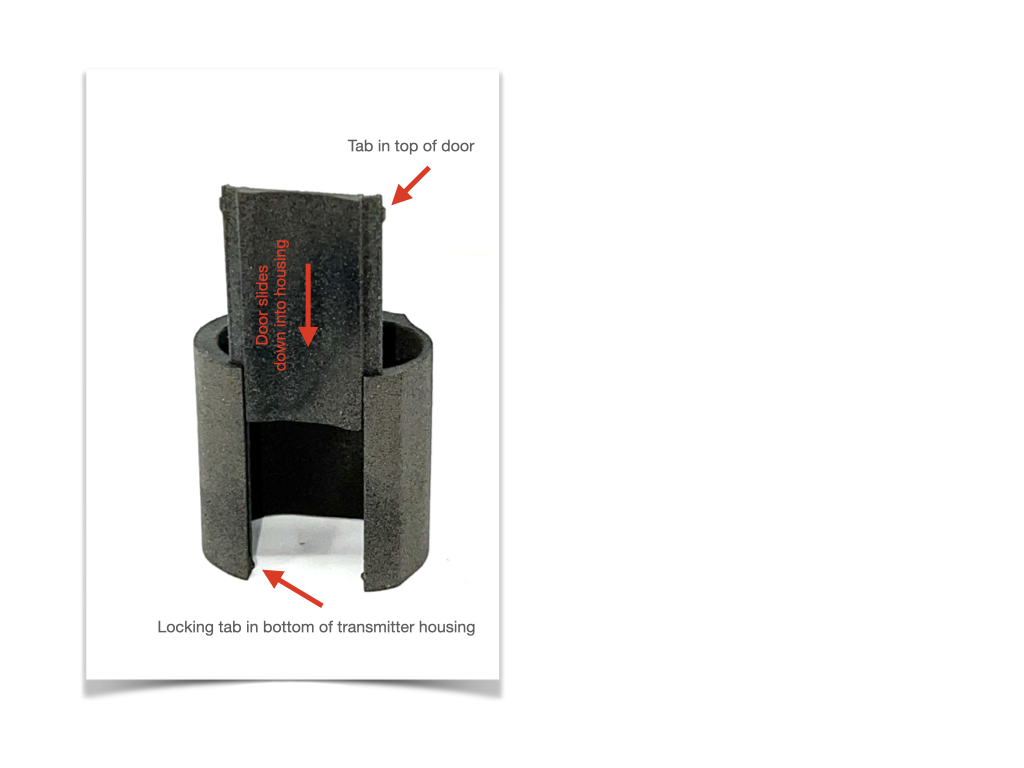
\includegraphics[width=1\textwidth,height=\textheight]{/Users/davidlapuma/Dropbox/CTT_Git/ctt_documentation/images/legband3.001.png}

Once locked into place the tag is secure and good to deploy. If you want
an extra bit of confidence you can place a small dab of super glue
between the upper and or lower locking tabs of the transmitter housing
before closing.

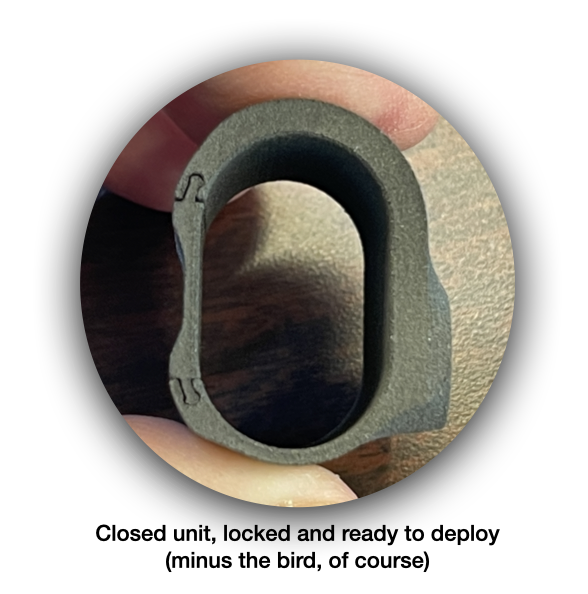
\includegraphics[width=0.5\textwidth,height=\textheight]{/Users/davidlapuma/Dropbox/CTT_Git/ctt_documentation/images/leg band user guide.003.png}

\hypertarget{removing-the-band}{%
\subsection{Removing the band}\label{removing-the-band}}

The bands are not meant to be removed once deployed, but if you need to,
the best way to do so is to cut the door section of the band. This will
allow the two halves of the door to fall away and you can simply slide
the leg out of the transmitter portion off of the band. If glue was used
you may have to cut along both sides of the door to remove a section
large enough to remove the tag from the leg.

\hypertarget{final-thoughts}{%
\subsection{Final Thoughts}\label{final-thoughts}}

This User Guide is a living document. Your experiences and input are
greatly appreciated so please don't hesitate to reach out to us
regarding what you'd like to see included here. You can submit your
suggestions and any errors to our \texttt{Customer\ Service\ Desk}
\href{https://celltracktech.com/support-customer-service-desk/}{here}
and we will work to incorporate them in future revisions. All material ©
Cellular Tracking Technologies, 2022.

\end{document}
